% !TeX spellcheck = fr_FR
%\part*{Annexes}
%\addcontentsline{toc}{chapter}{Annexes} % Adding toc entry

%%% COMMENT THESES LINES IF YOU DO NOT USE DEDICATED TOC FOR ANNEXES

%%% /COMMENT THESES LINES IF YOU DO NOT USE DEDICATED TOC FOR ANNEXES
%\pagecolor{asparagus}
%\afterpage{\nopagecolor}
%\begin{center}
%\textit{Imprimer idéalement cette page sur une page de couleur.}
%\textit{Chaque annexe doit commencer sur une nouvelle page et doit être numérotée : Annexe 1 puis Annexe 2, etc.}
%\end{center}

\begin{appendices}
	
\stopcontents[default]
\resumecontents[annexes]
	
\chapter{Annexe A : Architecture LSTMB sans TFR}
\label{app:1}

\section{Architecture}

\begin{figure}[H]
\centering
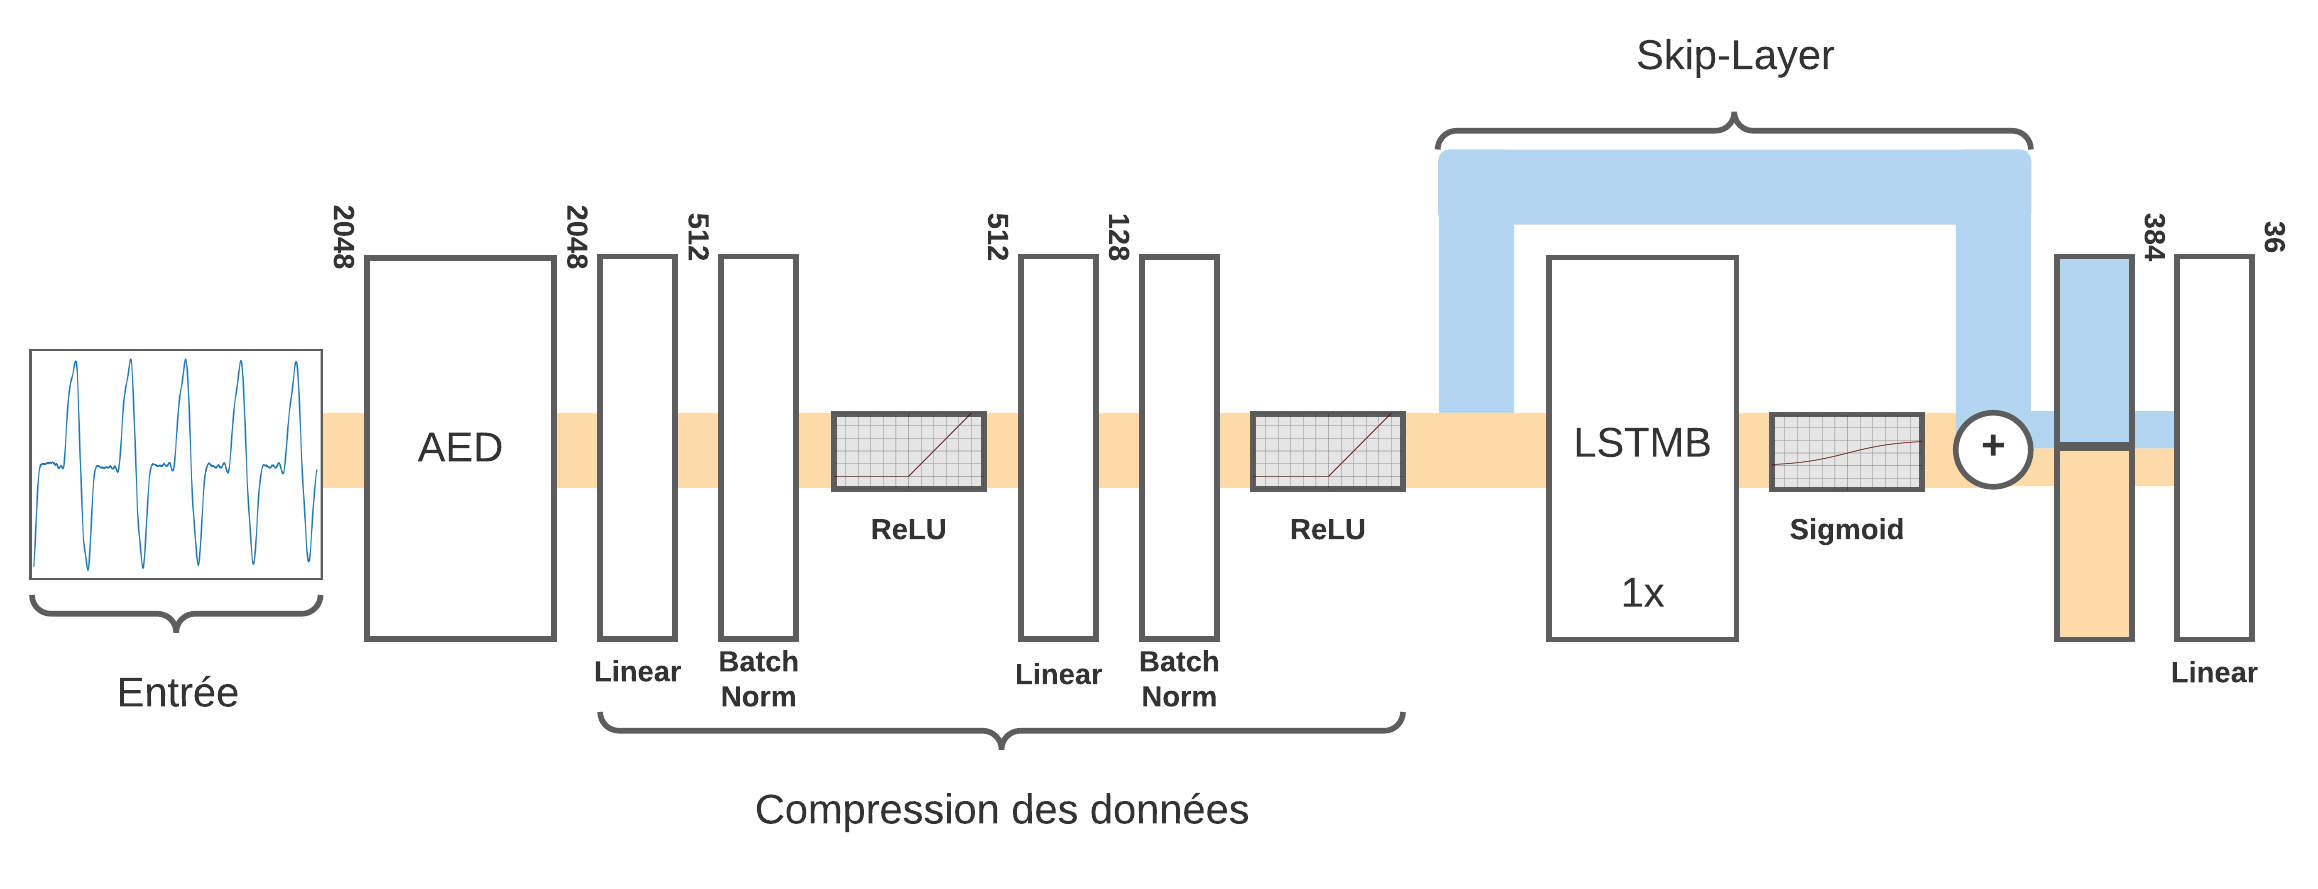
\includegraphics[width=1.1\linewidth,angle=-90,origin=c]{lstmb_no_fft}
\caption[]{Architecture LSTMB sans TFR. Source : Réalisé par \textsc{Küenzi} Jean-Daniel}
\label{fig:lstmb_no_fft}
\end{figure}

\section{Matrice de confusion sur l'ensemble de validation}

\begin{figure}[H]
\centering
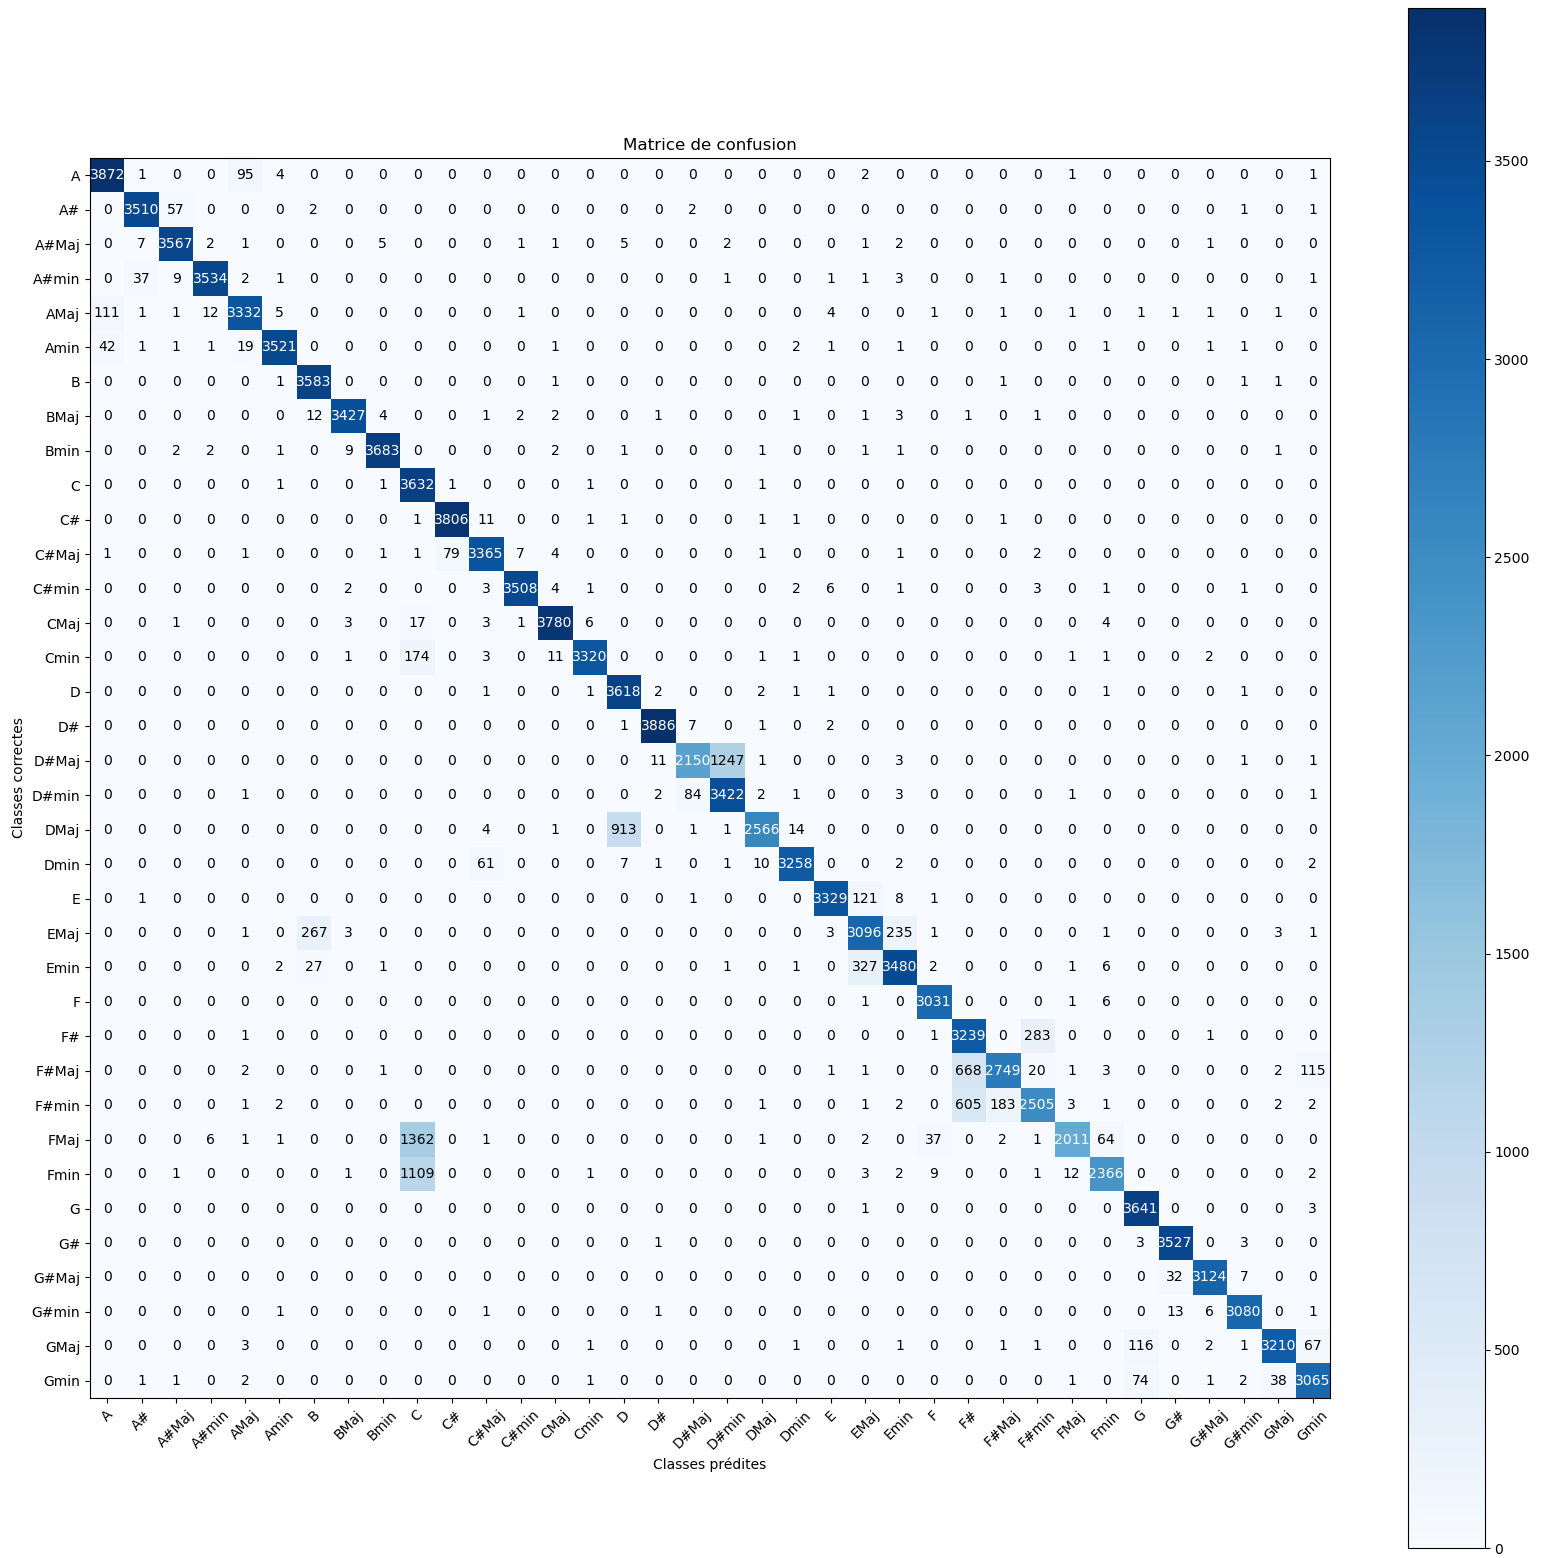
\includegraphics[width=1\linewidth]{cm_lstmb_no_fft}
\caption[]{Matrice de confusion pour l'architecture LSTMB sans TFR. Source : Réalisé par \textsc{Küenzi} Jean-Daniel}
\label{fig:cm_lstmb_no_fft}
\end{figure}	

\chapter{Annexe B : Architecture PMC sans TFR}
\label{app:2}

\section{Architecture}

\begin{figure}[H]
	\centering
	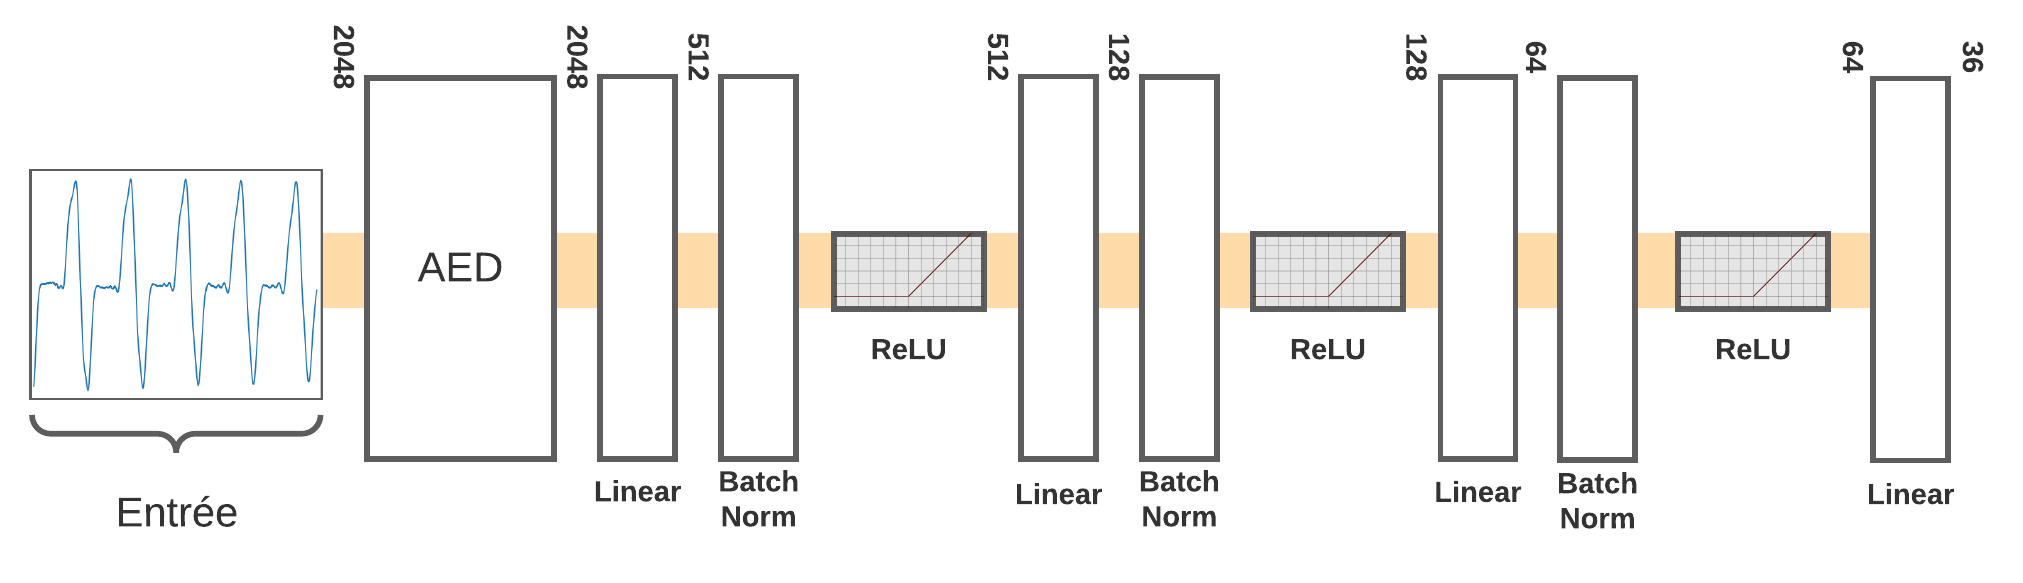
\includegraphics[width=1.1\linewidth,angle=-90,origin=c]{mlp_no_fft}
	\caption[]{Architecture PMC sans TFR. Source : Réalisé par \textsc{Küenzi} Jean-Daniel}
	\label{fig:mlp_no_fft}
\end{figure}

\section{Matrice de confusion sur l'ensemble de validation}

\begin{figure}[H]
\centering
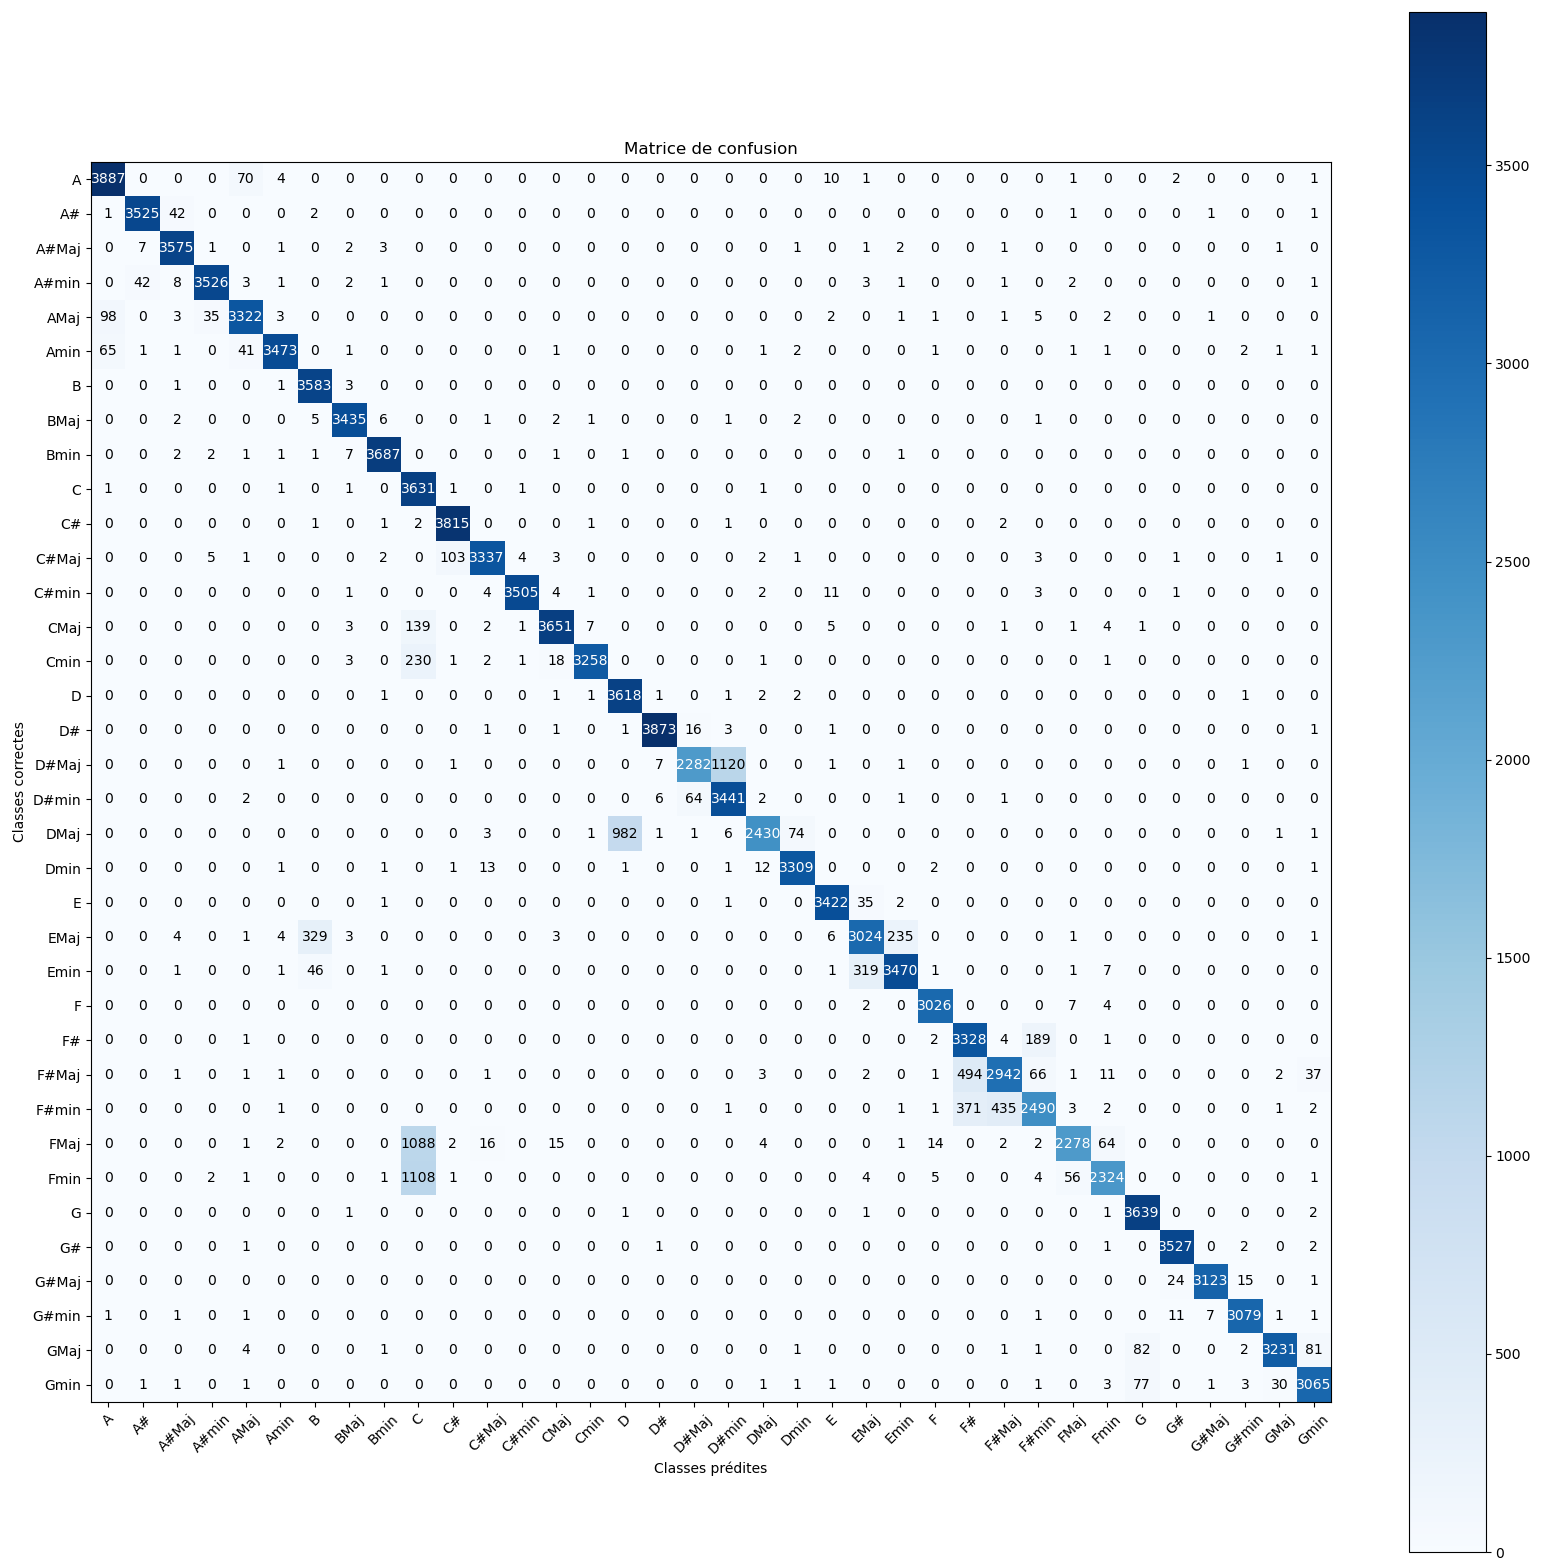
\includegraphics[width=1\linewidth]{cm_mlp_no_fft}
\caption[]{Matrice de confusion pour l'architecture PMC sans TFR. Source : Réalisé par \textsc{Küenzi} Jean-Daniel}
\label{fig:cm_mlp_no_fft}
\end{figure}	

\chapter{Annexe C : Architecture RNC sans TFR}
\label{app:3}

\section{Architecture}

\begin{figure}[H]
	\centering
	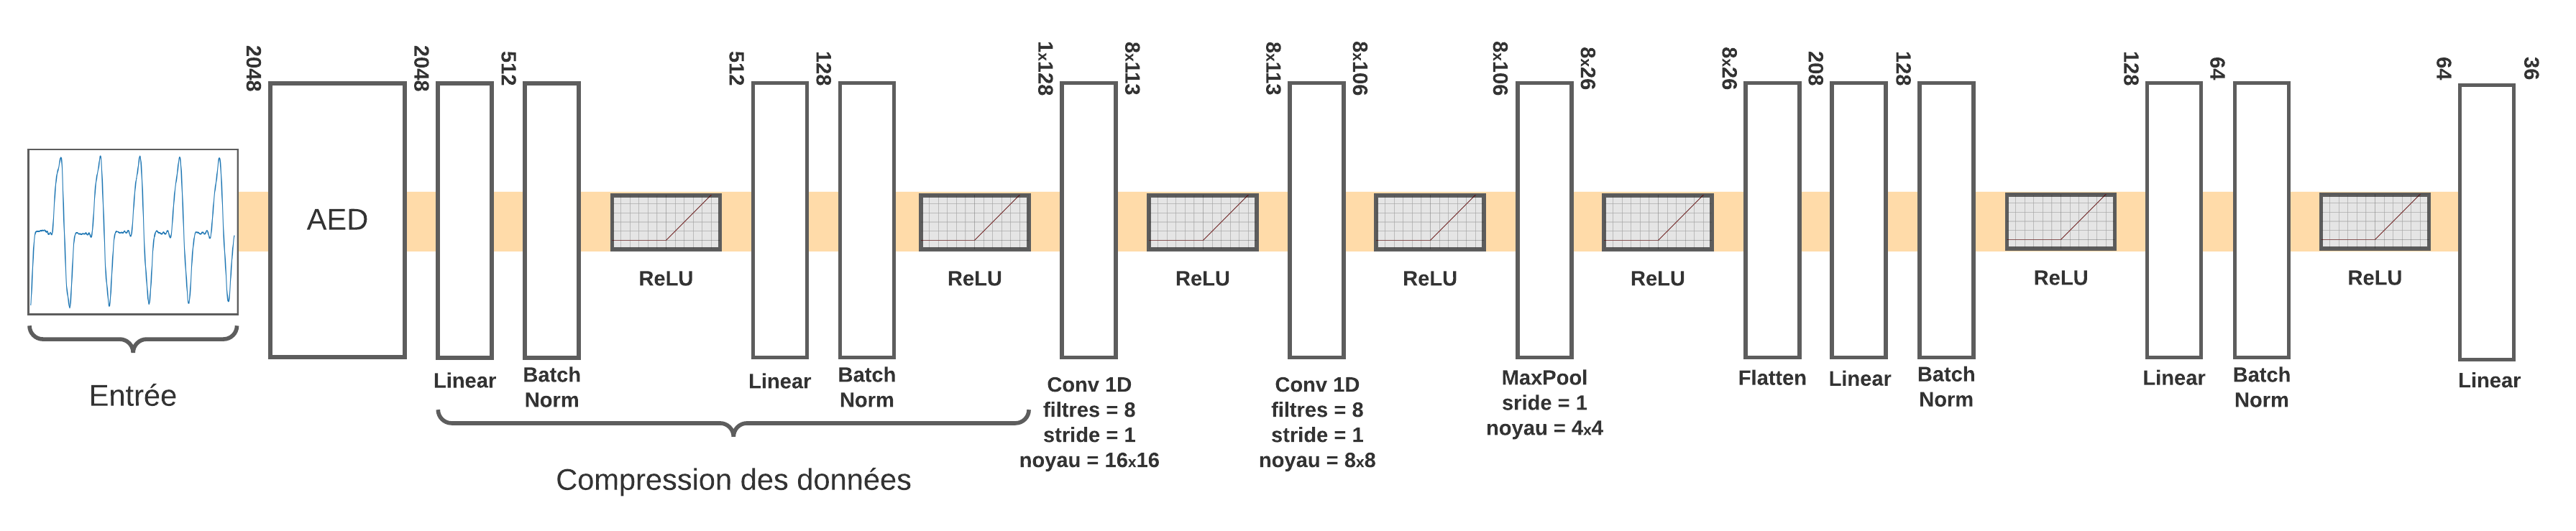
\includegraphics[width=1.1\linewidth,angle=-90,origin=c]{cnn_no_fft}
	\caption[]{Architecture RNC sans TFR. Source : Réalisé par \textsc{Küenzi} Jean-Daniel}
	\label{fig:cnn_no_fft}
\end{figure}

\section{Matrice de confusion sur l'ensemble de validation}

\begin{figure}[H]
\centering
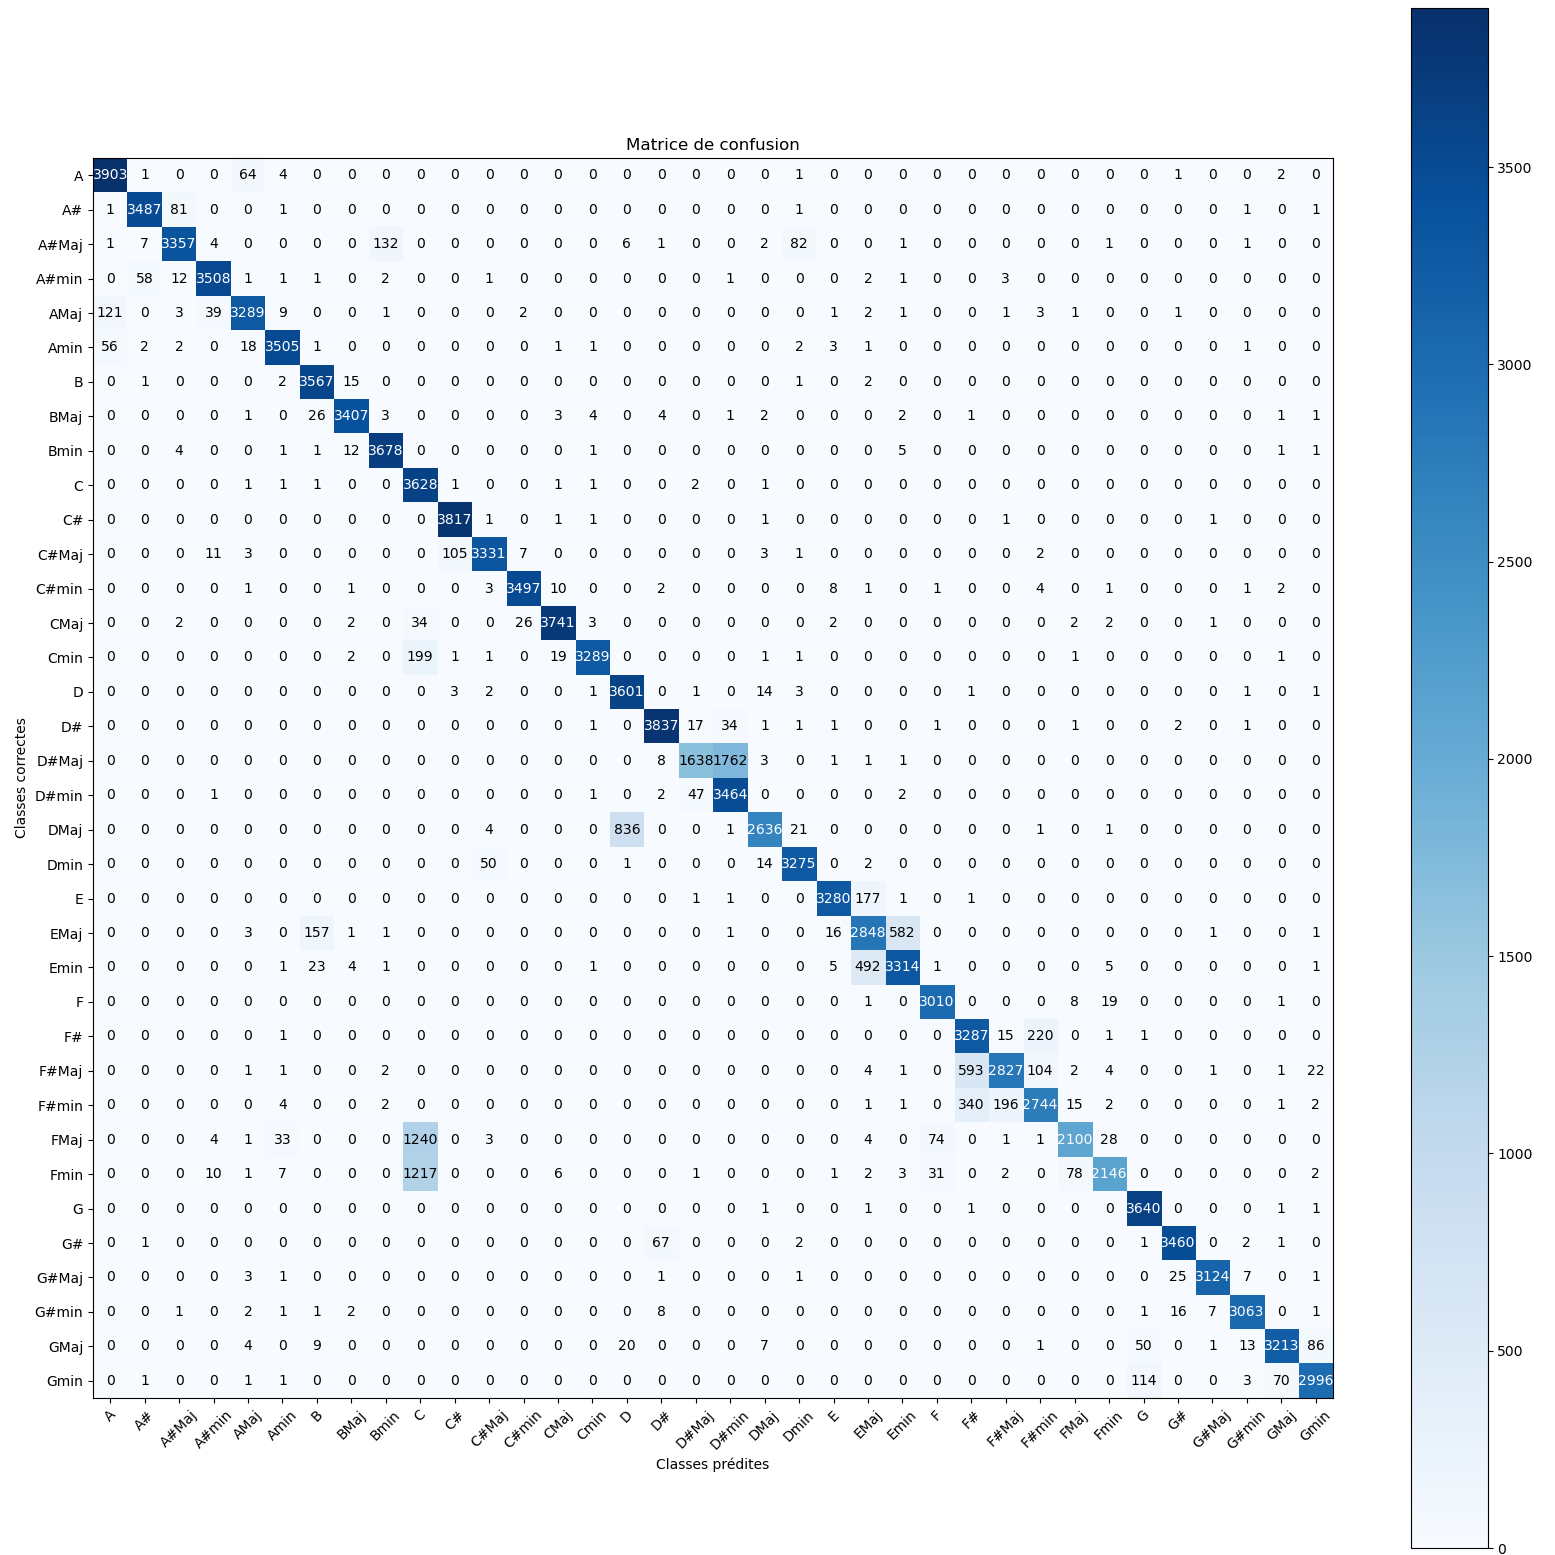
\includegraphics[width=1\linewidth]{cm_cnn_no_fft}
\caption[]{Matrice de confusion pour l'architecture RNC sans TFR. Source : Réalisé par \textsc{Küenzi} Jean-Daniel}
\label{fig:cm_cnn_no_fft}
\end{figure}

\chapter{Annexe D : Prédiciton de l'architecture PMC sur le fichier FMaj2 de l'ensemble de validation}
\label{app:4}

\begin{figure}[H]
	\centering
	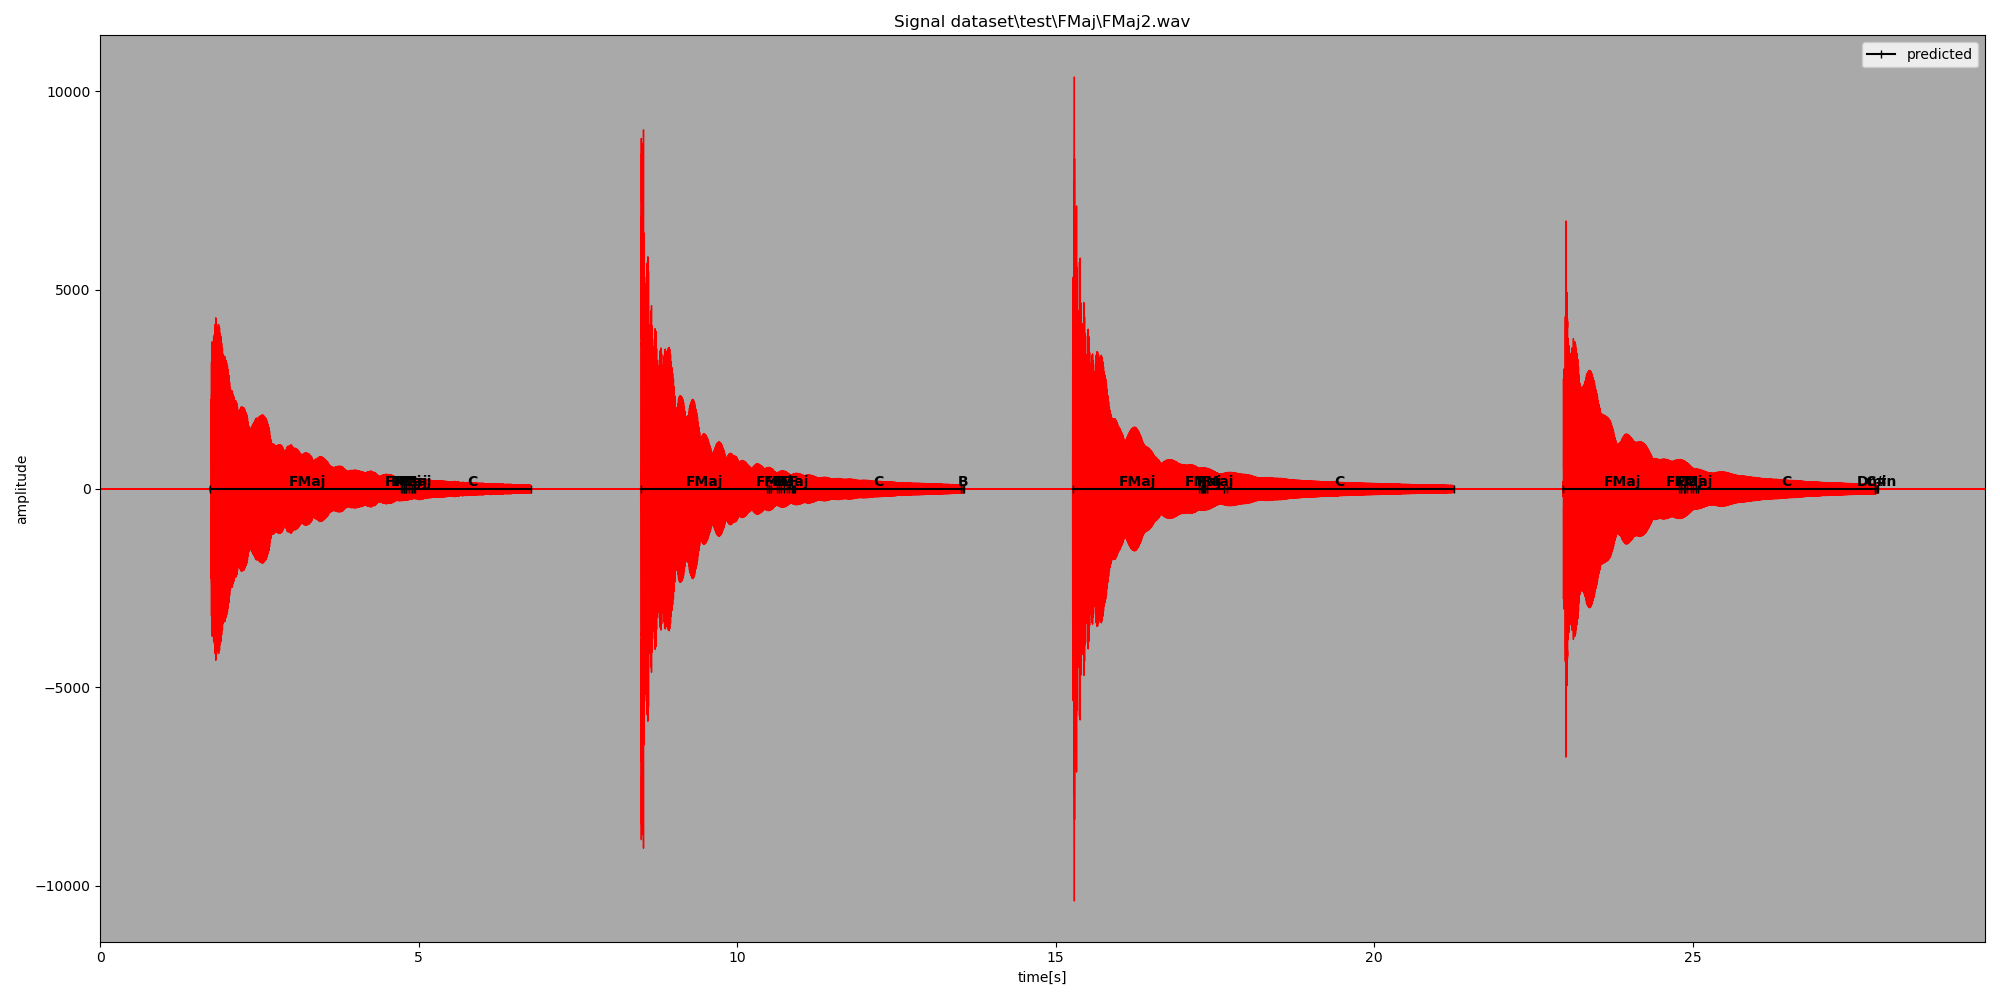
\includegraphics[width=1.2\linewidth,angle=-90,origin=c]{predict_FMaj2}
	\caption[]{Prédiction de l'architecture PMC sur le fichier FMaj2.wav du dataset de test. Source : Réalisé par \textsc{Küenzi} Jean-Daniel}
	\label{fig:predict_FMaj2}
\end{figure}

\chapter{Annexe E : Comparaison du spectre de Fourier de C\sh Maj et Dmin dans la même octave}
\label{app:5}

\begin{figure}[H]
	\centering
	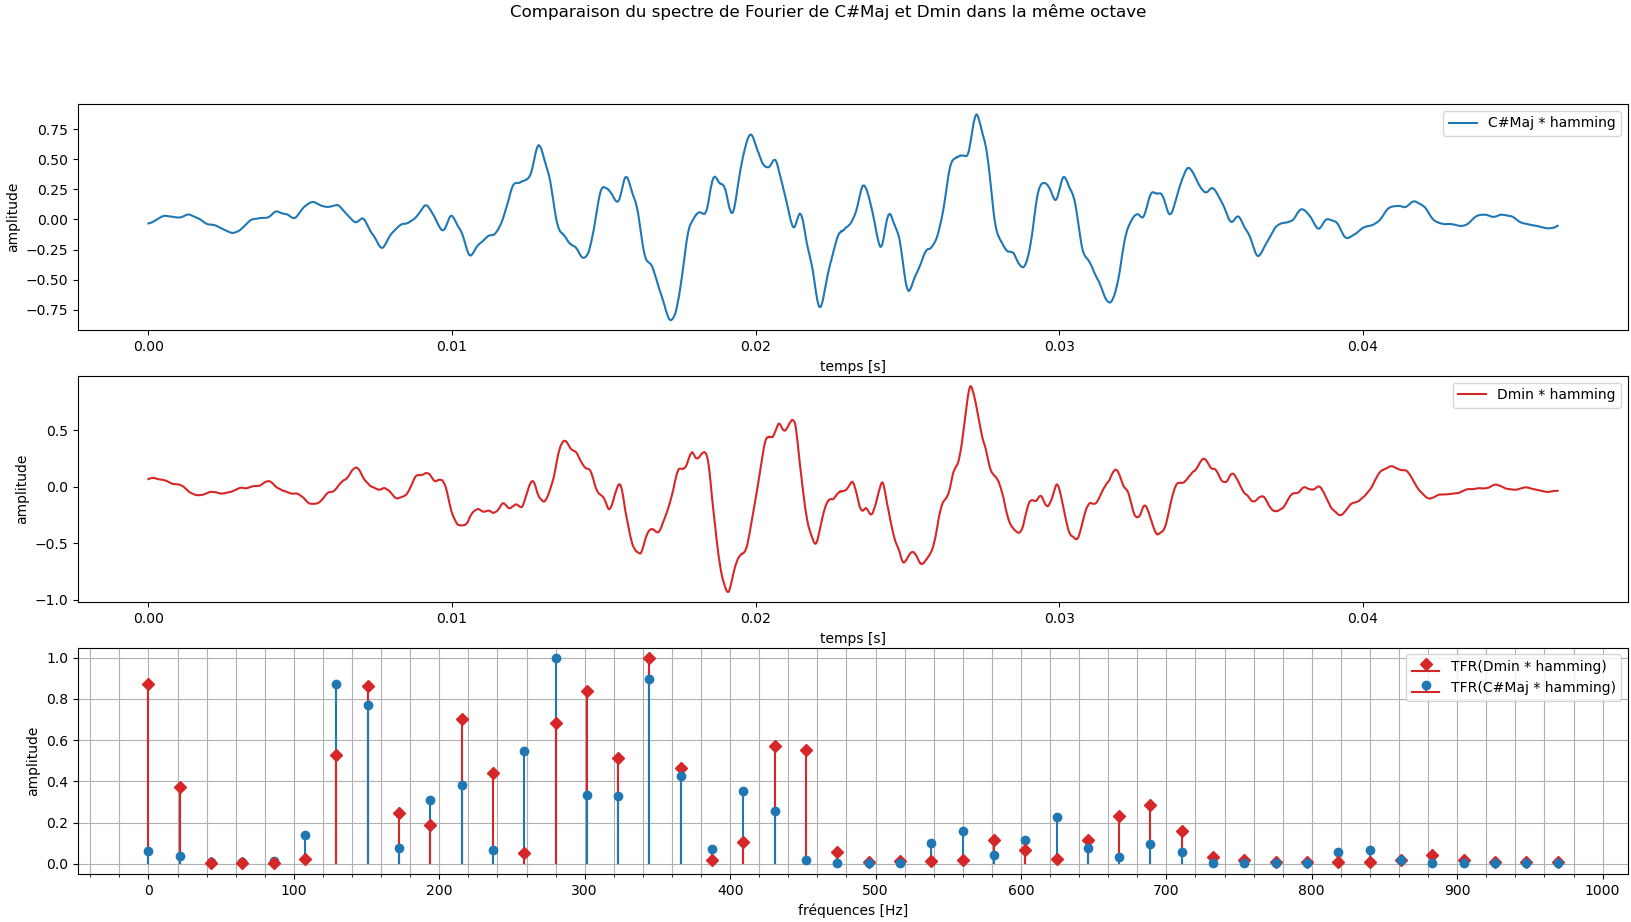
\includegraphics[width=1\linewidth]{fft_comp_chords_diff}
	\caption[]{Comparaison du spectre de Fourier de C\sh Maj et Dmin dans la même octave. Source : Réalisé par \textsc{Küenzi} Jean-Daniel}
	\label{fig:fft_comp_chords_diff}
\end{figure}

%%% COMMENT THESES LINES IF YOU DO NOT USE DEDICATED TOC FOR ANNEXES
\stopcontents[annexes]
\resumecontents[default]
%%% /COMMENT THESES LINES IF YOU DO NOT USE DEDICATED TOC FOR ANNEXES
\end{appendices}